
\subsubsection{UCS 7 - Monitoraggio degli accessi effettuati}

\begin{figure}[h]
	\centering
	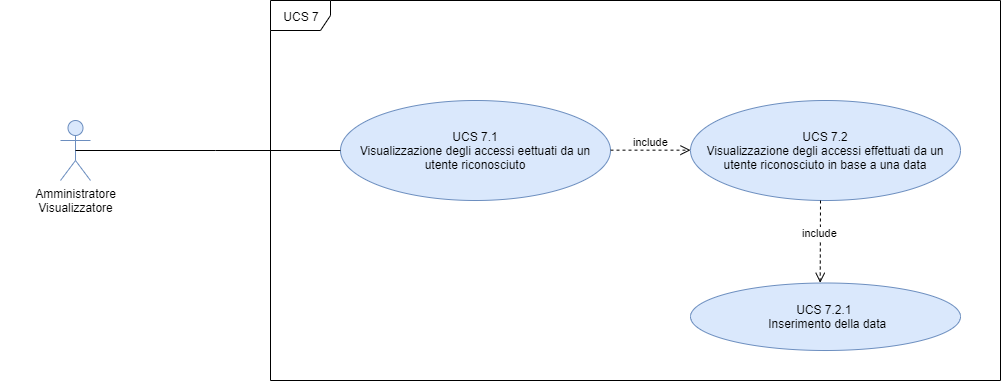
\includegraphics[scale=0.33]{Sezioni/UseCase/Immagini/UCS7.png}
	\caption{UCS 7 - Monitoraggio degli accessi effettuati}
\end{figure}

\begin{itemize}
\item \textbf{Attori primari:} Amministratore visualizzatore
\item \textbf{Precondizione:} L'amministratore dispone di almeno un'\glo{organizzazione}.
\item \textbf{Postcondizione:} L'amministratore ha monitorato gli accessi effettuati dagli utenti riconosciuti presso l'organizzazione.
\item \textbf{Scenario principale:} L'amministratore, dopo aver selezionato l'\glo{organizzazione}, accede alla funzionalità di visualizzazione della \glo{lista degli accessi} per monitorare gli utenti.
\end{itemize}

\subsubsection{UCS 7.1 - Visualizzazione degli accessi effettuati da un utente riconosciuto presso l'organizzazione}

\begin{figure}[h]
	\centering
	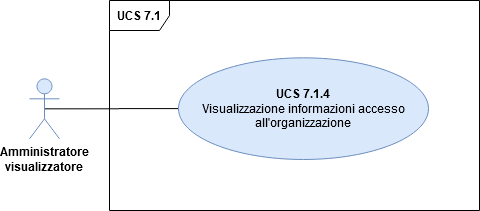
\includegraphics[scale=0.5]{Sezioni/UseCase/Immagini/UCS7.1.png}
	\caption{UCS 7.1 - Visualizzazione degli accessi effettuati da un utente riconosciuto presso l'organizzazione}
\end{figure}

\begin{itemize}
	\item \textbf{Attori primari:} Amministratore visualizzatore
	\item \textbf{Precondizione:} L'amministratore ha effettuato l'accesso alla funzionalità di monitoraggio degli accessi effettuati.
	\item \textbf{Postcondizione:} L'amministratore ha visionato la lista con gli accessi di un utente riconosciuto presso l'\glo{organizzazione}.
	\item \textbf{Scenario principale:} L'amministratore esegue la procedura per visualizzare lo \glo{storico degli accessi} effettuati presso l'\glo{organizzazione} desiderata da un utente riconosciuto.\\
	L'amministratore può selezionare un luogo all'interno dell'\glo{organizzazione} per monitorare gli accessi dell'utente al suo interno [UCS 7.2].
	\item \textbf{Flusso di eventi:}
	\begin{enumerate}
		\item L'amministratore seleziona un utente preciso da una lista contente tutti i utenti riconosciuti dell'\glo{organizzazione};
		\item L'amministratore visiona una lista con tutti gli accessi effettuati dall'utente selezionato presso l'\glo{organizzazione};
		\item L'amministratore visiona per ogni accesso le sue informazioni.
	\end{enumerate}
\end{itemize}

\subsubsection{UCS 7.1.4 - Visualizzazione informazioni accesso all'organizzazione}
\begin{itemize}
	\item \textbf{Attori primari:} Amministratore visualizzatore
	\item \textbf{Precondizione:} L'amministrazione sta visionando un accesso all'\glo{organizzazione}.
	\item \textbf{Postcondizione:} L'amministratore visiona le informazioni relative all'accesso effettuato.
	\item \textbf{Scenario principale:} Viene visualizzato il \glo{timestamp} di ingresso, di uscita e il tempo di permanenza presso l'\glo{organizzazione}.
\end{itemize}

\subsubsection{UCS 7.2 - Visualizzazione degli accessi effettuati da un utente riconosciuto presso un luogo all'interno dell'organizzazione}

\begin{figure}[h]
	\centering
	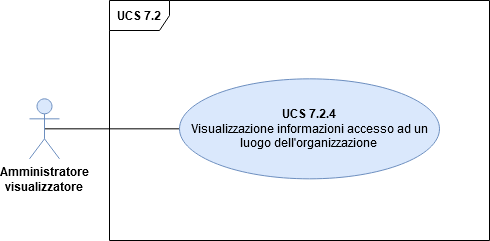
\includegraphics[scale=0.5]{Sezioni/UseCase/Immagini/UCS7.2.png}
	\caption{UCS 7.2 - Visualizzazione degli accessi effettuati da un utente riconosciuto presso un luogo all'interno dell'organizzazione}
\end{figure}

\begin{itemize}
	\item \textbf{Attori primari:} Amministratore visualizzatore
	\item \textbf{Precondizione:} L'amministratore ha effettuato l'accesso alla funzionalità di monitoraggio degli accessi effettuati.
	\item \textbf{Postcondizione:} L'amministratore ha visualizzato la lista con gli accessi di un utente riconosciuto presso un luogo all'interno dell'\glo{organizzazione}.
	\item \textbf{Scenario principale:} L'amministratore esegue la procedura per visualizzare lo \glo{storico degli accessi} effettuati presso un luogo all'interno dell'\glo{organizzazione} desiderata da un utente riconosciuto.
	\item \textbf{Flusso di eventi:}
	\begin{enumerate}
		\item L'amministratore seleziona un utente preciso da una lista contente tutti i utenti riconosciuti dell'\glo{organizzazione};
		\item L'amministratore visiona una lista con tutti gli accessi effettuati dall'utente selezionato presso il luogo dell'\glo{organizzazione};
		\item L'amministratore visiona per ogni accesso le sue informazioni.
	\end{enumerate}
\end{itemize}

\subsubsection{UCS 7.2.4 - Visualizzazione informazioni accesso ad un luogo dell'organizzazione}
\begin{itemize}
	\item \textbf{Attori primari:} Amministratore visualizzatore
	\item \textbf{Precondizione:} L'amministratore sta visionando un accesso ad un luogo dell'\glo{organizzazione}.
	\item \textbf{Postcondizione:} L'amministratore visiona le informazioni relative all'accesso effettuato.
	\item \textbf{Scenario principale:} Viene visualizzato il \glo{timestamp} di ingresso, di uscita e il tempo di permanenza presso il luogo dell'\glo{organizzazione}.
\end{itemize}

\subsubsection{UCS 7.4 - Ordinamento per data della lista degli accessi presso un'organizzazione o un suo luogo}
\begin{itemize}
    \item \textbf{Attori primari:} Amministratore visualizzatore
    \item \textbf{Precondizione:} L'amministratore seleziona la visualizzazione della lista degli accessi ordinata per data.
    \item \textbf{Postcondizione:} L'amministratore ottiene la \glo{lista degli accessi} riordinata \glo{per data}.
    \item \textbf{Scenario principale:} Ordinamento per data della lista degli accessi in un determinato ordine.
\end{itemize}

\subsubsection{UCS 7.4.1 - Ordinamento per data decrescente della lista degli accessi presso un'organizzazione o un suo luogo}
\begin{itemize}
	\item \textbf{Attori primari:} Amministratore visualizzatore
	\item \textbf{Precondizione:} L'amministratore seleziona la visualizzazione della lista degli accessi ordinata per data decrescente.
	\item \textbf{Postcondizione:} L'amministratore ottiene la \glo{lista degli accessi} riordinata \glo{per data in ordine decrescente}.
	\item \textbf{Scenario principale:} Ordinamento per data decrescente della lista degli accessi.
	\item \textbf{Generalizzazione:}
	\begin{enumerate}
		\item UCS 7.4 - Ordinamento per data della lista degli accessi presso un'organizzazione o un suo luogo.
	\end{enumerate} 
\end{itemize}

\subsubsection{UCS 7.4.2 - Ordinamento per data crescente della lista degli accessi presso un'organizzazione o un suo luogo}
\begin{itemize}
    \item \textbf{Attori primari:} Amministratore visualizzatore
    \item \textbf{Precondizione:} L'amministratore seleziona la visualizzazione della lista degli accessi ordinata per data crescente.
    \item \textbf{Postcondizione:} L'amministratore ottiene la \glo{lista degli accessi} riordinata \glo{per data crescente}.
    \item \textbf{Scenario principale:} Ordinamento per data crescente della lista degli accessi.
    \item \textbf{Generalizzazione:}
	\begin{enumerate}
		\item UCS 7.4 - Ordinamento per data della lista degli accessi presso un'organizzazione o un suo luogo.
	\end{enumerate}
\end{itemize}

\subsubsection{UCS 7.5 - Ricerca degli accessi presso un'organizzazione o un suo luogo in un giorno specifico}
\begin{itemize}
    \item \textbf{Attori primari:} Amministratore visualizzatore
    \item \textbf{Precondizione:} L'amministratore sta visualizzando lo storico accessi di un utente riconosciuto.
    \item \textbf{Postcondizione:} L'amministratore ottiene la lista di accessi effettuati nel giorno selezionato.
    \item \textbf{Scenario principale:} Ricerca degli accessi presso un'organizzazione o un suo luogo di un'organizzazione in un giorno specifico.
\end{itemize}